\documentclass[letterpaper]{article} 
\usepackage{pgfplots}
\usepackage{scalefnt} %用于设置字体
\usepgfplotslibrary{fillbetween}

\definecolor{color1}{RGB}{145,30,180}
\definecolor{color2}{RGB}{245,130,48}
\definecolor{color3}{RGB}{230,25,75}


\begin{document}

\begin{figure}[t!]	
\centering
\resizebox{0.8\columnwidth}{!}{  %用于修改图片大小
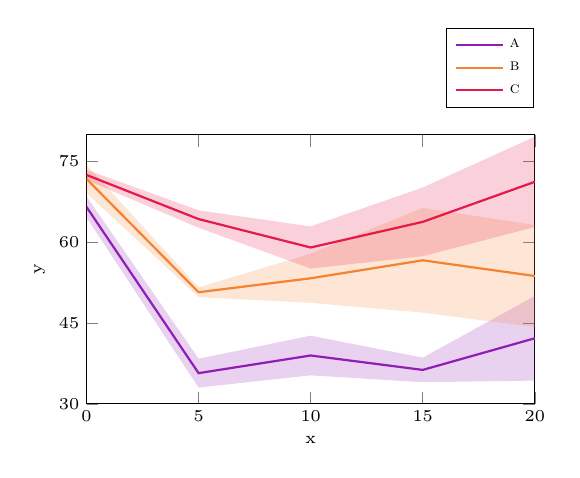
\begin{tikzpicture}
\footnotesize
\scalefont{0.7} %设置字体大小
\begin{axis}[
width=8cm, height=5cm,  %设置长和宽
ymin=30, ymax=80,
ytick={30,45,60,75},
ylabel style={text width=0.3\columnwidth,align=center}, 
xlabel= x,
ylabel = y,
width=0.6\columnwidth, 
xmin=0,xmax=20,
xtick={0,5,10,15,20},
ylabel near ticks,
legend style={at={(0.9,1.1)},anchor=south},
]

% 下界1
\addplot[draw=none,mark=none,name path=SeqSeqOneLower,forget plot] coordinates{
(0,64.62)
(5,33.03)
(10,35.30)
(15,34.03)
(20,34.32)
 };
% 上界1    
 \addplot[draw=none,mark=none,name path=SeqSeqOneUpper,forget plot] coordinates{
(0,68.54)
(5,38.40)
(10,42.67)
(15,38.59)
(20,50.05)
 };     
%下界1与上界1之间填充
\addplot [fill=color1,opacity=0.2,forget plot] fill between[of=SeqSeqOneLower and SeqSeqOneUpper];
% 绘制折线1     
 \addplot[color=color1,style={ thick}] coordinates { 
 (0,66.58)
(5,35.71)
(10,38.99)
(15,36.31)
(20,42.19)
}; 
\addlegendentry{\textsc{a}} % 设置名称1
      
% 下界2          
 \addplot[draw=none,mark=none,name path=SeqSeqLower,forget plot] coordinates{
(0,69.19)
(5,49.82)
(10,48.77)
(15,46.94)
(20,44.27)
};
% 上界2 
\addplot[draw=none,mark=none,name path=SeqSeqUpper,forget plot] coordinates{
(0,74.39)
(5,51.66)
(10,57.90)
(15,66.40)
(20,63.23)
};     
%下界2与上界2之间填充     
\addplot [fill=color2,opacity=0.2,forget plot] fill between[of=SeqSeqLower and SeqSeqUpper];
% 绘制折线2
\addplot[color=color2,style={ thick}] coordinates { 
(0,71.79)
(5,50.74)
(10,53.33)
(15,56.67)
(20,53.75)
}; 
\addlegendentry{\textsc{b}}
     
% 下界3    
\addplot[draw=none,mark=none,name path=FullGoldLower,forget plot] coordinates{
(0,71.57)
(5,62.72)
(10,55.14)
(15,57.42)
(20,62.86)
};
% 上界3     
\addplot[draw=none,mark=none,name path=FullGoldUpper,forget plot] coordinates{
(0,73.49)
(5,65.95)
(10,62.96)
(15,70.2)
(20,79.64)
 };     
%下界3与上界3之间填充    
\addplot [fill=color3,opacity=0.2,forget plot] fill between[of=FullGoldLower and FullGoldUpper];
% 绘制折线3
\addplot[color=color3,style={ thick}] coordinates { 
(0,72.53)
(5,64.33)
(10,59.05)
(15,63.81)
(20,71.25)
}; 
\addlegendentry{\textsc{c}}
        
\end{axis}

\end{tikzpicture}
}
\caption{Line chart with error bar}
\label{fig:1}
\end{figure}  

\end{document}
